\documentclass{article}

\usepackage{graphicx} % Required for inserting images
\usepackage{amsmath} % Required for flexibility in mathematical equations
\usepackage{amssymb} % Required for certain math symbols e.g. E[.]
\usepackage{natbib} % Required for bibliography and citations
\usepackage{enumitem} % Required to remove gap between items in list
\usepackage{tikz}

\title{Modelling and optimising the housing of homeless populations: ten month PhD review}
\author{Graham Burgess}
\date{October 2024}

\begin{document}

\maketitle

\begin{abstract}
Modelling and optimisation are popular tools for supporting resourcing and capacity decisions in healthcare and homeless settings. We show how deterministic optimisation with a fluid flow model can support long-term capacity planning for a homeless care setting in the San Francisco Bay Area, California. Models of multi fidelity, including stochastic simulation, are available in this setting, and the solution space is integer-ordered. We therefore explore both multi fidelity and integer-ordered simulation optimisation methods and discuss potential research contributions at the intersection of these active fields of research.
\end{abstract}

\section{Introduction}

Homelessness is a growing problem faced by communities worldwide. An example is Alameda County in the San Francisco Bay area, California, where approximately $8000$ people experienced homelessness in $2021$ alone. Decision makers within these communities typically have some leverage over how relevant resources are allocated to help alleviate homelessness. In Alameda County, the local government must split their resources between emergency shelter and permanent social housing. Shelter is relatively cheap and quick to set up. It provides a safer alternative to street homelessness but does not provide a stable long-term living situation for its residents. Permanent social housing is more expensive than shelter and can take longer to set up, but it does offer the stable long-term living situationd that homelessness people need to improve their quality of life. Building capacity to alleviate homelessness takes time, especially since funds are typically available in varying amounts from year to year. Decision makers in communities like Alameda County must therefore make good time-varying capacity planning decisions to reduce homelessness now and in the future. \newline

Operational research (OR) methods offer helpful tools to support such public sector decision-making. Optimisation helps decision-making by looking for a feasible solution which performs best across a (potentially infinite) set of alternative feasible solutions. To do this, a model of the performance of a solution is needed, and the quality of the model affects the quality of the subsequent optimisation results. We can model the homelessness care system as a queue. Homeless people must wait for permanent social housing to become available. Some of those in the queue for social housing can be accommodated in shelter, while the rest will be street homeless. Once a housing `server' becomes availabe, a resident may stay their for some time (in some cases, the rest of their lives) before they ultimately leave the system. \newline

The most accurate model of this queueing system is a high-fidelity stochastic simulation model. In this case, one can only estimate the performance of a solution and the subsequent optimisation falls in the realm of simulation optimisation (SO). There are different SO methods for different types of problem (which we later discuss) but the issue of limited computational resources pervades all SO methods. This issue stems from from the fact that a stochastic simulation is typically computationally expensive to run, and many simulation replications are required to be confident of a solution's performance, given the associated uncertainty. \newline

As is common in queueing systems, lower fidelity models such as analytical queueing models offer a computationally cheaper alternative to stochastic simulation. They also offer helpful alternative perspectives on the dynamics of a queueing system. The drawback is that these models are typically less accurate, given the necessary assumptions which must be made. If one only uses a low-fidelity deterministic model to evaluate the performance of a solution, optimisation falls in the realm of deterministic optimisation. Performing this deterministic optimisation can be a helpful first step in the decision-making process. However, there is more we can do with our low fidelity models. Multi-fidelity simulation optimisation (MFSO) enables low-fidelity models to be used alongside high fideltiy stocahstic simulation in a SO algorithm which reduces the computational burden and therefore enables an optimal solution to be found more efficiently. Novel MFSO methods will be the main topic of this PhD research. \newline

This document is organised as follows: in Section \ref{lit-rev} we briefly review relevant literature on modelling and optimisation in homeless care settings and healthcare settings. There are many similarities between these two and the latter is more widely studied in the literature. We also review relevant SO methods including MFSO. In Sections \ref{models} and \ref{do} we discuss the main content of the PhD research to date. Section \ref{models} introduces three models of multi-fidelity for homeless care systems. Section \ref{do} introduces an optimisation formualation which addresses the time-varying capacity planning problem and we solve this problem in a determinsitc setting. In Section \ref{uncert} we discuss how different types of uncertainty affect our decision-making process, and this discussion motivates the need for simulation optimisation. In Section \ref{mfso} we discuss relevant interesting gaps in the current MFSO literature which the remainder of this PhD research seeks to address.

\section{Literature Review} \label{lit-rev}

\subsection{Modelling and optimisation in healthcare settings}

Modelling hospital waiting lists using stochastic simulation e.g. \cite{wood2022supporting} and using stocks and flows e.g. \cite{worthington1991hospital}. Optimisation such as \cite{argyris2022fair} who balance efficiency and fairness in healthcare provision. 

\subsection{Modelling and optimisation in homeless care settings}

Simulation modelling of homeless care system in Alameda County \citep{singham2023discrete} and of shelters for runaway homeless youths (RHYs) \citep{kaya2022discrete}. Optimisation such as \cite{kaya2022improving} who minimise the cost of matching demand with supply for RHYs who require beds and support services.

\subsection{Simulation optimisation (SO)}

\subsubsection{Overview of SO methods}

\begin{itemize}[noitemsep]
\item Discrete SO: ranking \& selection, adaptive random search, integer-ordered.
\item Continuous SO: sample average approx, stochastic approx, meta models.
\end{itemize}

\subsubsection{Integer-ordered SO methods}
\begin{itemize} [noitemsep]
    \item Retrospective search with piecewise-linear interpolation and neighborhood enumeration (R-SPLINE) \citep{wang2013integer}.
    \item Discrete Stochastic Approximation \citep{lim2012stochastic}
    \item Gaussian Markov Random Fields \citep{l2019gaussian}
\end{itemize}

\subsubsection{Multi fidelity SO methods}

\begin{itemize}[noitemsep]
\item Using deterministic optimisation results to begin simulation optimisation e.g. \cite{jian2015introduction}.
\item Ordinal transformation with optimal sampling \citep{xu2016mo2tos}.
\item Modelling the error of a low-fidelity model
\begin{itemize}[noitemsep]
\item Polynomial error terms e.g. \cite{chong2018simulation}.
\item Gaussian Process error terms e.g. \cite{huang2006sequential}.
\end{itemize}
\item Multi-fidelity Expensive Black Box (Mf-EBB) Optimisation
\end{itemize}

\section{Models of multi-fidelity} \label{models}

Here we introduce three models for homeless care systems from low- to high-fidelity. Our low-fidelity model is a fluid flow model, which assumes housing servers are always busy and treats flow in and out of the system like a liquid with a continuous-valued volume. Our medium-fidelity model is an $M_t/M/h_t$ queueing model which relaxes the server-always-busy assumption. We incorporate stochasticity and using a Markov chain analysis we can compute the expected number of people housed, sheltered and unsheltered at some point in time, given initial conditions. Our high-fidelity model is a discrete-event simulation model. Here, as well as caputuring stochasticity we are able to model additional real-world processes such as the conversion of shelter to housing, delays between houses being vacated and re-occupied by others and non-Markovian service time distributions. We now discuss each model in turn.

\tikzstyle{server} = [rectangle, rounded corners, minimum width=0cm, minimum height=1cm,text centered, draw=black, fill=teal!30]
\tikzstyle{empty} = [rectangle, draw=none, fill=none]
\tikzstyle{arrow} = [thick,->,>=stealth]
\begin{figure} 
  \begin{center}
    \begin{tikzpicture}
      \node (start) [empty] {};
      \node (shelter) [empty, right of=start, xshift=2cm] {};
      \node (housing) [server, right of=shelter, xshift=2.2cm] {Housing};
      \node (end) [empty, right of=housing, xshift=2.1cm] {};
      \draw [arrow] (start) -- node [above] {Unsheltered \hspace{0.1cm} Sheltered} (housing);
      \draw [arrow] (housing) -- node [above] {}(end);  
      \draw[dashed] (3.5,-1) -- (3.5,1);
    \end{tikzpicture}
    \caption{Simple queueing system} \label{fig:simple-q}
  \end{center}
\end{figure}

Figure \ref{fig:simple-q} illustrates a simple queueing system which we model with a fluid flow model.

This section introduces a fluid flow queueing model which tracks the number of housed, sheltered, and unsheltered clients over time.   The two main inputs to the model are a changing arrival rate over time, and a housing service rate which changes as housing is built.  Additionally, the amount of shelter space available to support the queue for housing may change over time.  This models the dynamics in Figure \ref{fig:simple-q}.  Due to the current large queue for housing and continued inability for housing rates to keep up with arrivals to the system, the assumption that the servers will always be busy is not only reasonable, but significant enough to negate the usual assumptions of steady-state queueing behavior where the servers are idle with some positive probability.

In our fluid flow model we ignore the randomness in the arrival process and the service process for homeless people entering and leaving the homeless response system. Instead we assume that ``fluid" flows into the system continuously at a rate $\lambda(t)$ and flows out at  rate $\mu(t) = \mu_{0}h(t)$ where $\mu_{0}$ is the service rate of a single housing unit and $h(t)$ is the continuous-valued number of houses at time $t$. Given the initial number of people in the system $X_0$, at time $t$ we can calculate the subsequent number of people in the system, $X(t)$, as
%
\begin{equation*} \label{x_t}
X(t) = X_0 + \int_{0}^{t} \lambda(t) dt - \int_{0}^{t} \mu_0 h(t) dt.
\end{equation*}
%
We split the queue for housing into an unsheltered and a sheltered part. We denote by $s(t)$ the continuous-valued number of shelters at time $t$. The size of the unsheltered queue $u(t)$ is then 
%
\begin{align} 
u(t) & = X(t) - h(t) - s(t) \\
& = X_0 + \int_{0}^{t} \lambda(t) dt - \int_{0}^{t} \mu_0 h(t) dt - h(t) - s(t),
\label{u_t}
\end{align}
%
where we assume that capacities $h(t)$ and $s(t)$ are sufficiently small compared to the given arrival rate $\lambda(t)$ so that these resources are always full, and the use of a fluid flow model remains appropriate. In other words, the number of people housed and the number in shelter are the same as the housing and shelter capacities $h(t)$ and $s(t)$, respectively. In reality, there may be some friction in the system in that housing may be idle while units are experiencing turnover and the next person in the queue is being located, but this time can be incorporated into the service time distribution.

When analyzing the dynamics of the fluid flow model over a modeling horizon, we discretize time into days. We now let $\lambda_d, h^D_d, s^D_d$ and $u_d$ for all $d \in \{1,...,D\}$ be the discretized equivalents of $\lambda(t), h(t), s(t)$ and $u(t)$, respectively, where $D$ is the modeling horizon in days and is used as a superscript where we must later distinguish between daily and annual capacities. In order to evaluate our various objective functions (which we describe in Section \ref{do}) we typically approximate (\ref{u_t}) with the sum 
%
\begin{align} \label{u_t_discrete}
u_d & = X_0 + \sum_{d'=1}^{d} \lambda_{d'} \delta t - \sum_{d'=1}^{d} \mu_0 h^D_{d'} \delta t - h^D_d - s^D_d, 
\end{align}
where $\mu_0$ is the daily service rate of a single housing unit and the stepsize $\delta t = 1 \text{ day}$. In Figure \ref{fig:ut-illustrative} we give an illustrative example of the dynamics of $u_d$ given by our fluid flow model, calibrated using realistic inputs for $X_0, \mu_0$ and $\lambda_d, h^D_d, s^D_d$ for all $d \in \{1,...,D\}$ which we take directly from \cite{singham2023discrete}. 

\begin{figure}[h!]%[ut-illustrative]
    \centering
    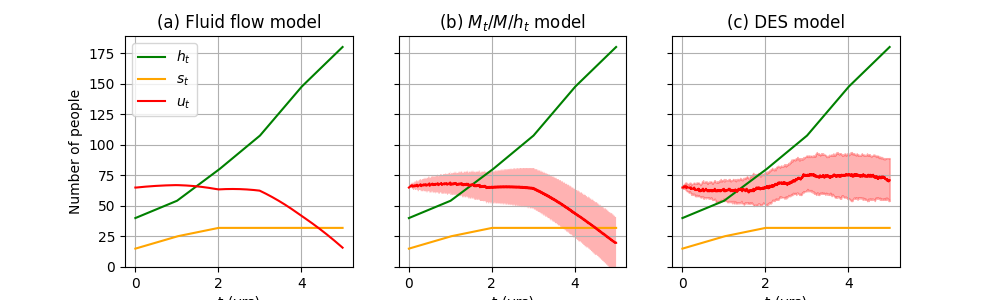
\includegraphics[scale=0.8]{u_t_example.png}
    \caption{Dynamics of $u_d$, $s^D_d$ and $h^D_d$. $X_0 = 12000$, $\mu_0 = 6.106 \times 10^{-4}$, Daily arrival rates $\lambda_d$ in each year: $10.0,11.9,13.1,13.1,11.8$.}
    \label{fig:ut-illustrative}
\end{figure}

Figure \ref{fig:ut-illustrative} shows an example of how one might come close to reaching functional zero in five years.  The level of housing investment steadily increases over time.  There is some initial increase in shelter, though in general there is less investment in shelter over the long term than in housing.  The unsheltered population is stabilized and then eventually decreases approaching zero.  The arrival rates $\lambda_d$ are projected based on a current estimate of 10/day, along with the assumption that arrivals will increase in the coming years due to repercussions of COVID-19.  Eventually, prevention methods will take effect and the arrival rate will hopefully decline \citep{hometogether2022}. The daily service rate $\mu_0$ is equivalent to the mean of a triangular distribution with lower limit $0 \text{ weeks}$, upper limit $400 \text{ weeks}$ and mode $300 \text{ weeks}$. 

In Section \ref{do} we will evaluate (\ref{u_t_discrete}) using annual housing and shelter capacity vectors $\boldsymbol{h} = \{h_t \hspace{0.1cm} \forall t \in 0,...,T\}$ and $\boldsymbol{s} = \{s_t \hspace{0.1cm} \forall t \in 0,...,T\}$ where $T$ is a time horizon in years. In this case we assume that any annual increase or decrease in capacity is spread evenly throughout the year, and (\ref{u_t_discrete}) becomes
%
\begin{align} \label{u_t_discrete_h_s_dependent}
u_d(\boldsymbol{h},\boldsymbol{s}) & = X_0 + \sum_{d'=1}^{d} \lambda_{d'} \delta t - \sum_{d'=1}^{d} \mu_0 h^D_{d'}(\boldsymbol{h}) \delta t - h^D_d(\boldsymbol{h}) - s^D_d(\boldsymbol{s}),
\end{align}
%
where 
%
\begin{align} \label{h_d}
h^D_d(\boldsymbol{h}) & = h_{\lfloor{\frac{d}{365}}\rfloor} + \frac{d-\lfloor\frac{d}{365}\rfloor}{365}(h_{\lceil{\frac{d}{365}}\rceil}-h_{\lfloor{\frac{d}{365}}\rfloor})
\end{align}
%
and
%
\begin{align} \label{s_d}
s^D_d(\boldsymbol{s}) & = s_{\lfloor{\frac{d}{365}}\rfloor} + \frac{d-\lfloor\frac{d}{365}\rfloor}{365}(s_{\lceil{\frac{d}{365}}\rceil}-s_{\lfloor{\frac{d}{365}}\rfloor}).
\end{align}
%
\section{Deterministic optimisation with low-fidelity model} \label{do}

\begin{itemize}[noitemsep]
\item Optimisation formulations
\item Numerical results
\end{itemize}

\section{Discussion of uncertainty} \label{uncert}

\begin{itemize}[noitemsep]
\item Stochastic uncertainty in homeless care problem (arrival/service processes).
\item Input model uncertainty: good input models for today cannot reliably predict future events.
\end{itemize}

\section{Potential contributions at intersection of integer-ordered and multi fidelity SO} \label{mfso}

\begin{itemize}[noitemsep]
\item Using low-fidelity models to quickly compute gradients in RSPLINE/DSA.
\item Adding prior information to GMRF using low-fidelity model.
\item Modelling errors of low fidelity models using GMRF.
\end{itemize}

\section{Conclusion}\label{conc}

\newpage

\bibliographystyle{apalike}
\bibliography{bibliography.bib}

\end{document}